\pagebreak

\paperwidth=\pdfpageheight
\paperheight=\pdfpagewidth
\pdfpageheight=\paperheight
\pdfpagewidth=\paperwidth
\headwidth=\textheight
%%\footerheight=\paperheight
\begingroup 
\vsize=\textwidth
\hsize=\textheight

\subsection{Gantt chart}
\label{ssec:gantt}

\begin{figure}[!ht]
\hspace{-1.5cm}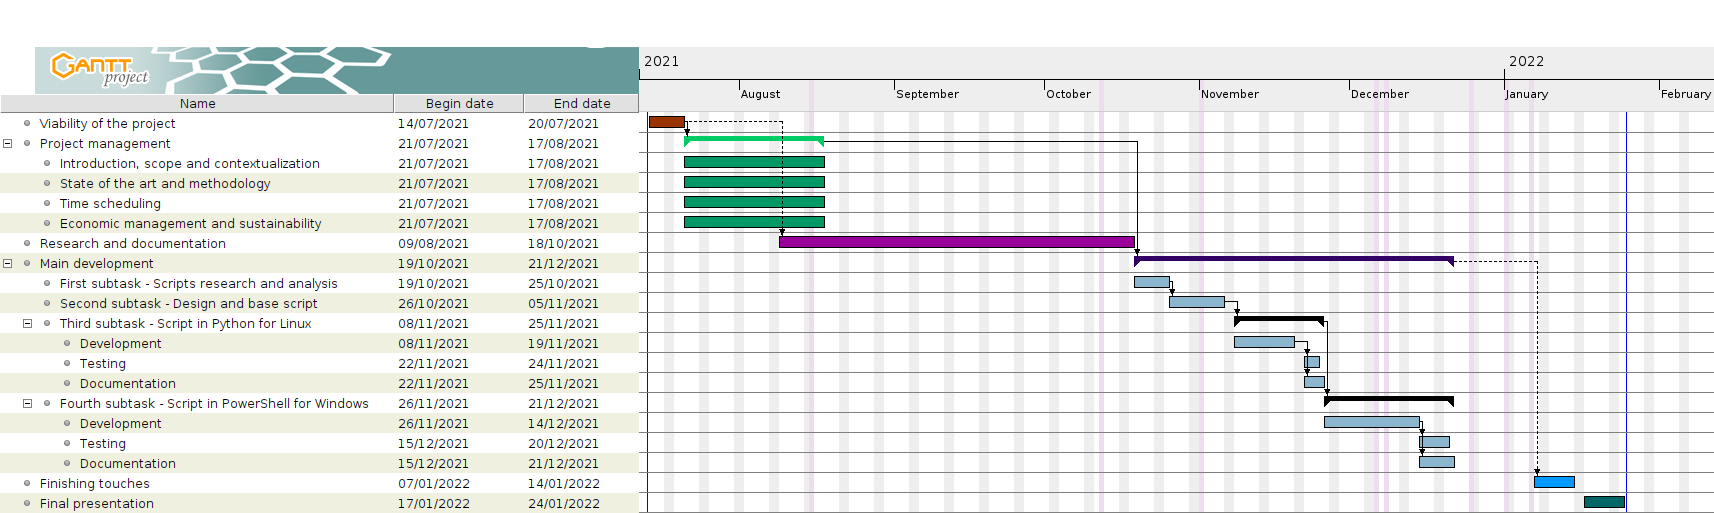
\includegraphics[width=27cm,trim={0 0 2.7cm 0},clip]{graphics/GanttChart}
\caption{Gantt chart created with GanttProject}
\end{figure}


\newpage

\subsection{PERT diagram}
\label{ssec:pert}

\begin{figure}[!ht]
\vspace{2cm}
\hspace{-0.5cm}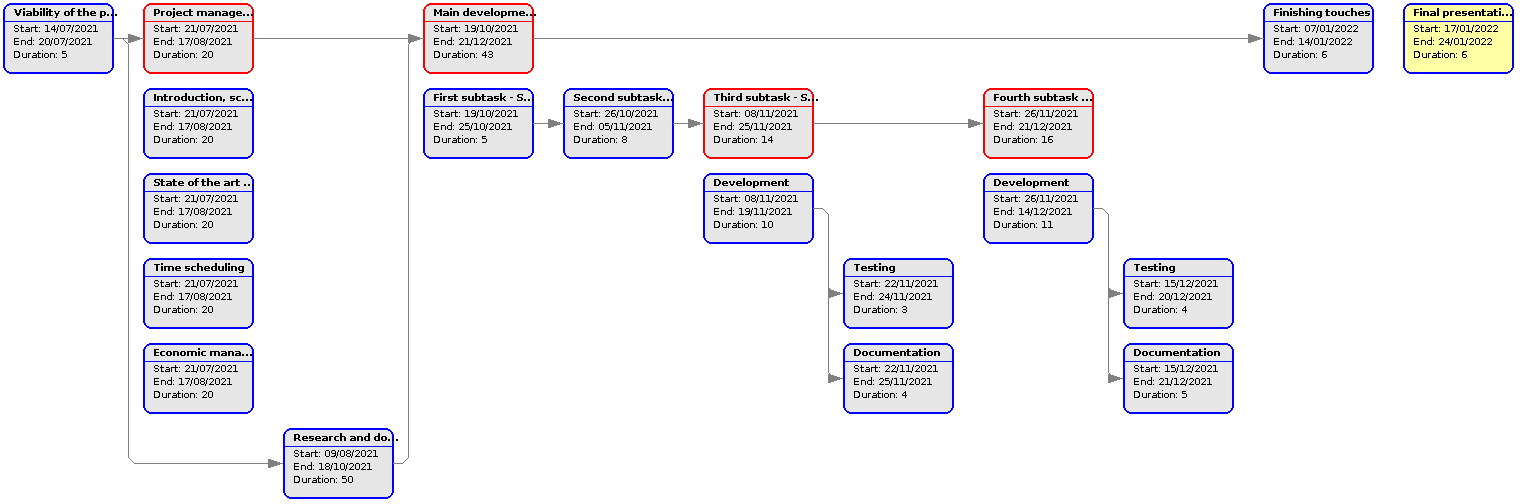
\includegraphics[width=25cm]{graphics/PERTChart}
\vspace{0.5cm}
\caption{PERT diagram based on the previous Gantt chart}
\end{figure}

\endgroup

\pagebreak

\paperwidth=\pdfpageheight
\paperheight=\pdfpagewidth
\pdfpageheight=\paperheight
\pdfpagewidth=\paperwidth
\headwidth=\textwidth